
\subsection{Size of the constraint set}

%Increasing the size of the constraint set $X$ impacts the running time,
%tree topology accuracy, and criterion scores for FastRFS-enhanced and 
%ASTRAL-enhanced. 
FastRFS-enhanced uses a larger constraint space than FastRFS-basic.
Table \ref{tab:set-x} shows the sizes of the constraint sets $X$ for
the five biological datasets that are added to the search spaces for
FastRFS-enhanced and ASTRAL-enhanced.

\begin{table*}
  \centering
  \begin{tabular}{c|rrrrr}
    Method             & Seabirds & Placental & Marsupial & THPL & CPL
    \\
    \hline 
    FastRFS-basic      & 1155     & 6907      & 10251     & 11109&
                                                                   20233
    \\
    FastRFS-enhanced      & 2485     & 12937      & 15443     & 17811&
                                                                   48313 \\    
  \end{tabular}
  \caption{Sizes of the set $X$ on biological datasets}
  \label{tab:set-x}
\end{table*}



\subsection{Commands}

Commands for the tree estimation software are provided below:

\paragraph{MulRF: }
We ran MulRF version 1.2 ten times,  and the tree with the
best optimization score was used. The command was:
\begin{verbatim}
MulRFSupertree -i <input file name> -o <output file name>
\end{verbatim}

\paragraph{PluMiST: }
We ran PluMiST version 1.1.  Since we found PluMiST's stopping
condition caused it to run for too long, we allowed PluMiST to run for
a limited amount of time (1 hour for 100-taxon simulated dataset; 5
hours for 500-taxon simulated dataset; 12 hours for the the seabird,
mammalian, and placental datasets, and 24 hours for the THPL
dataset). In all cases, this was at least as long as the other methods
took to run and in most cases substantially longer. Reported running
times are the times of the last iteration that successfully completed
before the cutoff. The command used for PluMiST was
\begin{verbatim}
python plumist.py -s <input file name> -o <output file name>
\end{verbatim}


\paragraph{MRL: }
We also ran matrix representation with likelihood (MRL), in which a
maximum-likelihood tree is estimated on an MRP matrix. We generated
MRP matrices with mrpmatrix, available at
\url{github.com/smirarab/mrpmatrix}:
\begin{verbatim}
mrpmatrix <input file> <output matrix file> -dna
\end{verbatim}
We estimated MRL trees with RAxML version 8.2.4 with command line 
\begin{verbatim}
RAxML -m BINGAMMA -p 12345 -n <run name> -s <matrix file>
\end{verbatim}

\paragraph{ASTRID:}
To run ASTRID, we used the command line
\begin{verbatim}
ASTRID -i <gene tree file> -o <output file>
\end{verbatim}

\paragraph{ASTRAL:}
To run ASTRAL, we used the command line
\begin{verbatim}
java -jar astral.4.7.8.jar -i <gene tree file> -o <output file>
\end{verbatim}
To run ASTRAL-enhanced, we used
\begin{verbatim}
java -jar astral.4.7.8.jar -i <gene tree file> -o <output file> -e
<extra trees>
\end{verbatim}
where the extra trees file contained the MRL tree or the MRL tree and
the ASTRID tree, depending on whether or not the ASTRID distance
matrix was complete.

\paragraph{FastRFS-basic: } 
To run FastRFS, we used the command line
\begin{verbatim}
wASTRAL -c FastRF  -g <gene tree file> -o <output file>
-a /path/to/astral.4.7.8.jar
\end{verbatim}

\paragraph{FastRFS-enhanced: }

To run the enhanced version of FastRFS, we used the
command line
\begin{verbatim}
wASTRAL -c FastRF  -g <gene tree file> -o <output file>
-a /path/to/astral.4.7.8.jar -e <extra trees> --extraextra
\end{verbatim}
%TODO: describe this
This runs the clade selection portion of ASTRAL three times to get the
constraint set. First, it runs with the input trees as gene trees and
the extra trees as extra trees. Second, it runs with the extra trees
as the gene trees. Finally, it runs with input and extra trees
combined as gene trees. The union of these outputs is used as the
clade set for FastRFS.
\clearpage

 \begin{figure*}
   \centering
   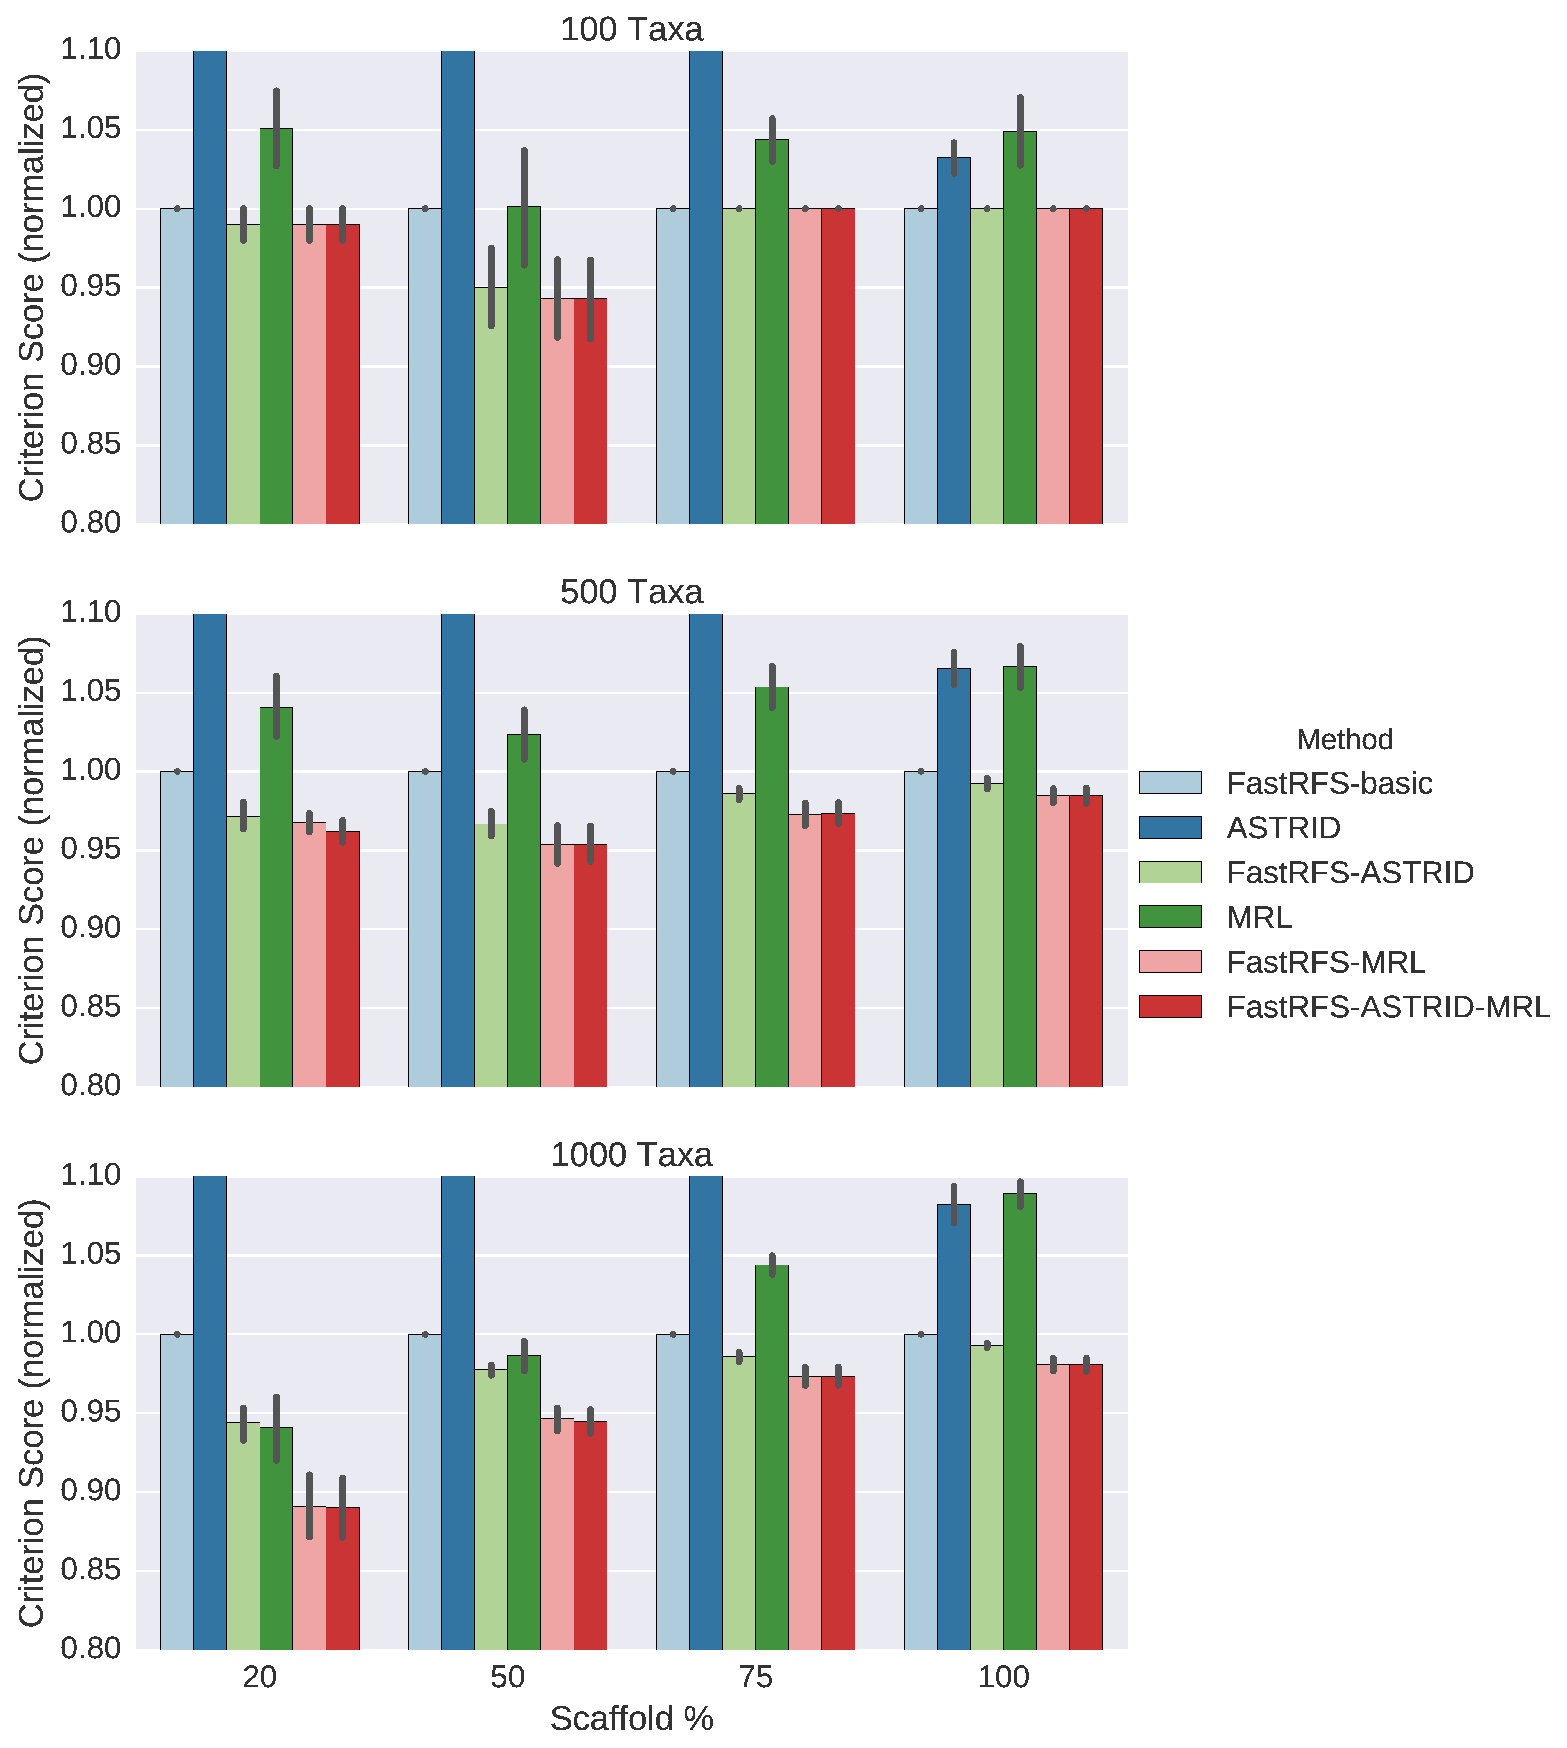
\includegraphics[width=\textwidth,height=0.6\textheight,keepaspectratio]{fastrfs-figs/smidgen-critscores-fastrfs-comparison.eps}  
   \caption{Comparison of FastRFS variants criterion scores on
     simulated data. Scores are normalized by dividing by the
     FastRFS-basic score; FastRFS-basic has a score of 1.}
   \label{fig:fastrfs-sup::sim-fastrfs-comp}
 \end{figure*}


 % \begin{figure*}
 %   \centering
 %   \includegraphics[width=\textwidth]{../../rfsupertree/analysis/smidgen-err-fastrfs-comparison}  
 %   \caption{Comparison of FastRFS variants topological errors on
 %     simulated data.}
 %   \label{fig:sim-fastrfs-comp}
 % \end{figure*}



 % \begin{figure*}
 %   \centering
 %   \includegraphics[width=\textwidth]{../../rfsupertree/analysis/smidgen-timing-fastrfs-comparison}  
 %   \caption{Comparison of FastRFS variants running times on simulated
 %     data. This does not take into account the additional time needed
 %     to run ASTRID and MRL. }
 %   \label{fig:sim-fastrfs-comp}
 % \end{figure*}


 \begin{figure*}
   \centering
   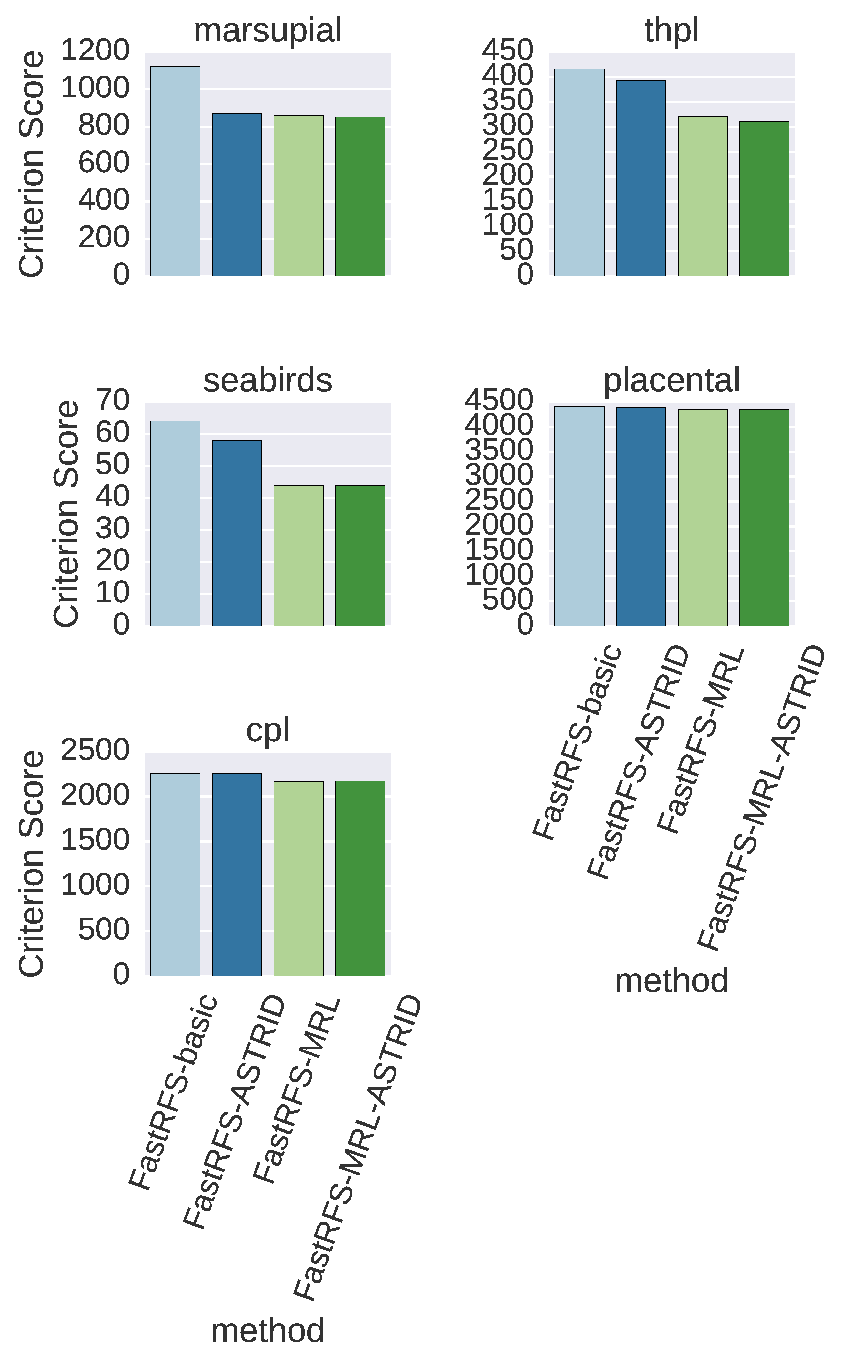
\includegraphics[width=\textwidth,height=0.9\textheight,keepaspectratio]{fastrfs-figs/bio-rfscores-fastrfs-comp.eps}
   \caption{Comparison of FastRFS variants on biological data}
   \label{fig:fastrfs-sup::bio-fastrfs-comp}
 \end{figure*}
